\section{Cluster Structures}

\begin{figure}[h]
 \centering
 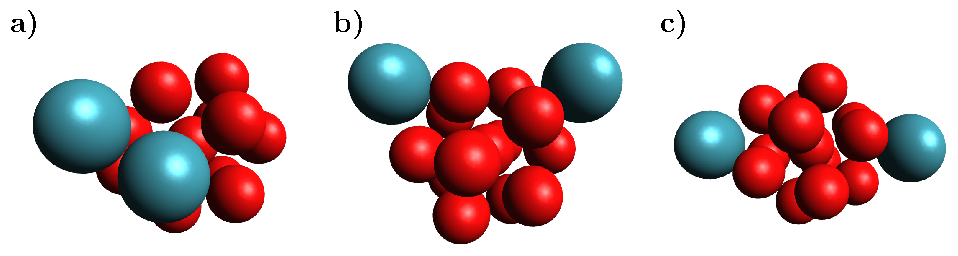
\includegraphics[width=8.5cm]{pics/cluster_2_overview.pdf}
 \caption{Cluster structures with 13 argon atoms and two additional xenon
          atoms on different surfaces of the argon icosahedron:
          \textbf{a)} closest possible \textbf{b)} middle \textbf{c)}
          furthest away.}
 \label{figure:cluster_2_overview}
\end{figure}



\begin{figure}[h]
 \centering
 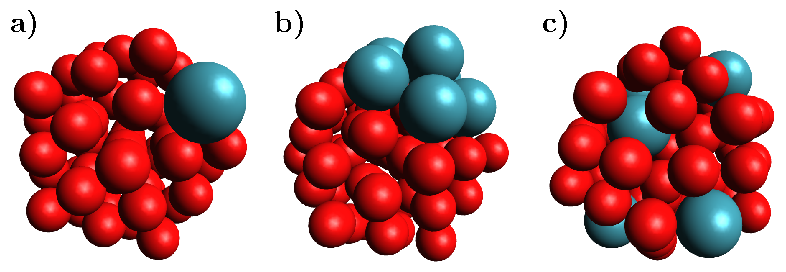
\includegraphics[width=8.5cm]{pics/cluster_3_overview.pdf}
 \caption{Cluster structures based on 55 atoms icosahedral cluster structure.
          \textbf{a)} 1 xenon atom on the surface of a 55 atoms icosahedral
          argon cluster. \textbf{b)} six xenon atoms inside a 55 atoms cluster
          grouped on one side. \textbf{c)} six xenon atoms distributed
          in a 55 atoms cluster. }
 \label{figure:cluster_3_overview}
\end{figure}
